% !TEX root = ../MuñozPedro_MT.tex
% =====================================================================
%  Sección: Encoder invariante al número de vértices (Deep Sets vs MLP)
%  Para incluir dentro del capítulo de Desarrollo Metodológico con:
%      % !TEX root = ../MuñozPedro_MT.tex
% =====================================================================
%  Sección: Encoder invariante al número de vértices (Deep Sets vs MLP)
%  Para incluir dentro del capítulo de Desarrollo Metodológico con:
%      % !TEX root = ../MuñozPedro_MT.tex
% =====================================================================
%  Sección: Encoder invariante al número de vértices (Deep Sets vs MLP)
%  Para incluir dentro del capítulo de Desarrollo Metodológico con:
%      % !TEX root = ../MuñozPedro_MT.tex
% =====================================================================
%  Sección: Encoder invariante al número de vértices (Deep Sets vs MLP)
%  Para incluir dentro del capítulo de Desarrollo Metodológico con:
%      \input{Capitulos/encoder_deepsets}
%
%  Requiere las librerías TikZ de abajo. Si compilas con \include de este
%  archivo, las \usetikzlibrary funcionan aquí; idealmente muévelas al
%  preámbulo de MuñozPedro_MT.tex junto a \usepackage{tikz}.
% =====================================================================
\usetikzlibrary{positioning,arrows.meta,fit,backgrounds,calc}

\section{Encoder invariante al número de vértices: de la MLP a Deep Sets}
\label{sec:deepsets}

La arquitectura LMI-Net descrita en la Sección~\ref{sec:arquitectura_lminet} fija el número
de vértices del polítopo en $N=2$. Esta sección aborda la limitación estructural que impide
generalizar a un $N$ arbitrario y propone como solución un \textit{encoder} de conjunto
invariante a permutación y a cardinalidad, basado en la arquitectura \textit{Deep
Sets}~\cite{zaheer2017deep}.

\subsection{La entrada es un conjunto, no un vector}
\label{subsec:entrada_conjunto}

Un sistema politópico queda descrito por el \textbf{conjunto} de sus $N$ vértices
$\{(A_i, B_i)\}_{i=1}^{N}$, con $A_i \in \mathbb{R}^{n_x \times n_x}$ y
$B_i \in \mathbb{R}^{n_x \times n_u}$. Cada vértice aporta, por tanto,
\begin{equation}
    d_v \;=\; n_x^2 + n_x\,n_u
\end{equation}
escalares; para la topología de estudio ($n_x=3$, $n_u=1$) esto es $d_v = 9 + 3 = 12$.

Resulta esencial notar una \textbf{asimetría estructural} entre la entrada y la salida del
mapa que la red debe aprender. La salida es el certificado $(Q, Y)$ codificado en el vector
$y$, cuya dimensión
\begin{equation}
    \dim y \;=\; \tfrac{n_x(n_x+1)}{2} + n_u\,n_x
    \label{eq:dim_y}
\end{equation}
\textbf{no depende de $N$} (vale $6+3=9$ para todo $N$), porque se busca \emph{una sola}
función de Lyapunov común $V(x)=x^\top Q^{-1} x$ y \emph{una sola} ganancia $K = Y Q^{-1}$
válidas simultáneamente para todos los vértices (estabilizabilidad cuadrática). Además, el
conjunto factible de la LMI es idéntico ante cualquier reordenamiento de los vértices: la
entrada es un \emph{conjunto}, no una secuencia. El mapa a aprender es entonces
\begin{equation}
    \{(A_i,B_i)\}_{i=1}^{N} \;\longmapsto\; (Q, Y),
\end{equation}
es decir, \emph{un conjunto de tamaño variable hacia un vector de tamaño fijo, invariante a
permutación}.

\subsection{El cuello de botella del backbone MLP}
\label{subsec:cuello_mlp}

El backbone original construye un único vector aplanando y concatenando todos los vértices,
\begin{equation}
    \mathbf{f} \;=\; \big[\,\mathrm{vec}(A_1),\,\mathrm{vec}(B_1),\,\dots,\,
    \mathrm{vec}(A_N),\,\mathrm{vec}(B_N)\,\big] \in \mathbb{R}^{N d_v},
    \label{eq:features_mlp}
\end{equation}
y lo procesa con una red densa cuya primera capa es una matriz
$W_1 \in \mathbb{R}^{h \times N d_v}$ (con $h$ el ancho oculto). Esta construcción acarrea
dos problemas insalvables para un $N$ variable:

\begin{enumerate}
    \item \textbf{Dependencia dimensional.} El tamaño de $W_1$ está atado a $N$: una red
    entrenada con $N=2$ posee $W_1 \in \mathbb{R}^{h\times 24}$ y no puede siquiera recibir
    la entrada de un sistema con $N=3$ ($\mathbb{R}^{h\times 36}$). En consecuencia, se
    requiere \emph{una arquitectura distinta por cada valor de $N$}.
    \item \textbf{Dependencia del orden.} La concatenación~\eqref{eq:features_mlp} asigna una
    columna de pesos distinta a cada posición; la red aprende parámetros específicos para
    ``la entrada $(1,1)$ de $A$ del vértice $1$'', otros para el vértice $2$, etc. Pero los
    vértices forman un conjunto, de modo que la red malgasta capacidad intentando aprender
    una invarianza a permutación que no se le garantiza.
\end{enumerate}

El relleno con ceros (\textit{zero-padding}) hasta un $N_{\max}$ fijo no resuelve nada: no
restaura la invarianza a permutación, inyecta vértices espurios $A=0,\,B=0$ que la red
interpreta como restricciones reales, y sigue sin poder extrapolar a $N > N_{\max}$.

\subsection{El encoder Deep Sets}
\label{subsec:deepsets}

La idea central de Deep Sets es cambiar la unidad de procesamiento: en vez de operar sobre el
conjunto aplanado, se aplica una misma función a \emph{cada vértice por separado} y se agregan
los resultados con una operación simétrica. El teorema de representación
de~\cite{zaheer2017deep} establece que toda función continua invariante a permutación admite
la forma
\begin{equation}
    f\big(\{x_1,\dots,x_N\}\big) \;=\; \rho\!\left( \frac{1}{N}\sum_{i=1}^{N} \phi(x_i) \right),
    \label{eq:deepsets}
\end{equation}
donde $\phi$ y $\rho$ son perceptrones multicapa. Concretamente, para cada vértice se forma
$x_i = [\mathrm{vec}(A_i),\,\mathrm{vec}(B_i)] \in \mathbb{R}^{d_v}$; una MLP compartida
$\phi:\mathbb{R}^{d_v}\!\to\!\mathbb{R}^{d}$ lo lleva a un embedding; estos se agregan por
promedio en $z\in\mathbb{R}^{d}$; y una MLP $\rho:\mathbb{R}^{d}\!\to\!\mathbb{R}^{\dim y}$
produce la propuesta $\hat y$ que alimenta la capa de proyección de Douglas--Rachford, la cual
se conserva \emph{sin modificación}. La Figura~\ref{fig:mlp_vs_deepsets} contrasta ambos
flujos.

\begin{figure}[ht]
\centering
\begin{subfigure}[b]{0.46\textwidth}
\centering
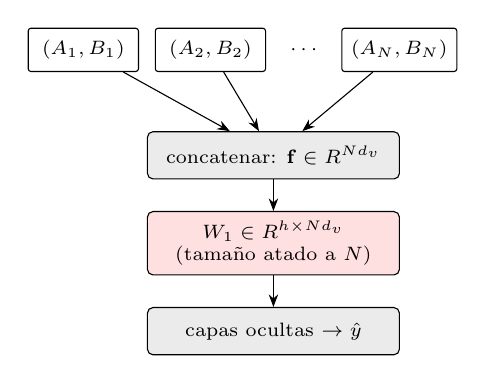
\begin{tikzpicture}[
    font=\scriptsize,
    box/.style={draw, rounded corners=1pt, minimum width=1.4cm, minimum height=0.55cm, align=center},
    op/.style={draw, fill=black!8, rounded corners=2pt, minimum width=3.2cm, minimum height=0.6cm, align=center},
    >={Stealth[length=1.6mm]}]
  \node[box] (v1) {$(A_1,B_1)$};
  \node[box, right=0.2cm of v1] (v2) {$(A_2,B_2)$};
  \node[right=0.18cm of v2] (vd) {$\cdots$};
  \node[box, right=0.18cm of vd] (vN) {$(A_N,B_N)$};
  \node[op, below=0.75cm of v2, xshift=0.8cm] (cat) {concatenar: $\mathbf{f}\in\mathbb{R}^{N d_v}$};
  \node[op, below=0.4cm of cat, fill=red!12] (w1) {$W_1\in\mathbb{R}^{h\times N d_v}$\\ (tama\~no atado a $N$)};
  \node[op, below=0.4cm of w1] (mlp) {capas ocultas $\to \hat y$};
  \draw[->] (v1) -- (cat); \draw[->] (v2) -- (cat);
  \draw[->] (vN) -- (cat);
  \draw[->] (cat) -- (w1); \draw[->] (w1) -- (mlp);
\end{tikzpicture}
\caption{Backbone MLP: una red por cada $N$.}
\label{fig:mlp}
\end{subfigure}
\hfill
\begin{subfigure}[b]{0.5\textwidth}
\centering
\begin{tikzpicture}[
    font=\scriptsize,
    box/.style={draw, rounded corners=1pt, minimum width=1.0cm, minimum height=0.55cm, align=center},
    phi/.style={draw, fill=blue!10, rounded corners=2pt, minimum width=1.0cm, minimum height=0.55cm, align=center},
    op/.style={draw, fill=black!8, rounded corners=2pt, minimum width=3.6cm, minimum height=0.6cm, align=center},
    >={Stealth[length=1.6mm]}]
  \node[box] (v1) {$x_1$};
  \node[box, right=0.45cm of v1] (v2) {$x_2$};
  \node[right=0.3cm of v2] (vd) {$\cdots$};
  \node[box, right=0.3cm of vd] (vN) {$x_N$};
  \node[phi, below=0.55cm of v1] (p1) {$\phi$};
  \node[phi, below=0.55cm of v2] (p2) {$\phi$};
  \node[phi, below=0.55cm of vN] (pN) {$\phi$};
  \node[op, below=0.7cm of p2, xshift=0.7cm, fill=green!12] (pool)
        {pooling (media): $z=\tfrac1N\sum_i \phi(x_i)$};
  \node[op, below=0.4cm of pool] (rho) {$\rho \to \hat y$};
  \draw[->] (v1) -- (p1); \draw[->] (v2) -- (p2); \draw[->] (vN) -- (pN);
  \draw[->] (p1) -- (pool); \draw[->] (p2) -- (pool); \draw[->] (pN) -- (pool);
  \draw[->] (pool) -- (rho);
  \node[draw, dashed, fit=(p1)(pN), inner sep=3pt,
        label={[font=\tiny]below:pesos compartidos}] {};
\end{tikzpicture}
\caption{Encoder Deep Sets: una red para todo $N$.}
\label{fig:deepsets}
\end{subfigure}
\caption{Comparación de los flujos de información. En la MLP (a), el número de vértices $N$
determina el tamaño de la primera capa $W_1$. En Deep Sets (b), la misma red $\phi$ se aplica
a cada vértice (pesos compartidos) y el \textit{pooling} colapsa el conjunto en un vector de
tamaño fijo; $N$ solo aparece en una operación sin parámetros.}
\label{fig:mlp_vs_deepsets}
\end{figure}

La Tabla~\ref{tab:transformaciones} detalla las transformaciones con sus dimensiones, para un
lote (\textit{batch}) de $B$ sistemas.

\begin{table}[ht]
\centering
\caption{Transformaciones del encoder Deep Sets (lote de $B$ sistemas).}
\label{tab:transformaciones}
\begin{tabular}{clc}
\toprule
Paso & Operación & Forma del tensor \\
\midrule
Entrada & $A_{\text{poly}},\,B_{\text{poly}}$ & $(B,N,n_x,n_x),\ (B,N,n_x,n_u)$ \\
1 & aplanar y concatenar por vértice & $(B,N,d_v)$ \\
2 & $\phi$ por vértice (pesos compartidos) & $(B,N,d)$ \\
3 & \textsc{pooling} (media sobre vértices) & $(B,d)$ \\
4 & $\rho$ & $(B,\dim y)$ \\
5 & desempaquetar a $(Q,Y)$ y proyectar (DR) & $(B,n_x,n_x),\ (B,n_u,n_x)$ \\
\bottomrule
\end{tabular}
\end{table}

El mecanismo preciso del paso~2 es el \textbf{peso compartido}: al aplicar una capa lineal
$\phi:\mathbb{R}^{d_v}\!\to\!\mathbb{R}^{d}$ a un tensor de forma $(B,N,d_v)$, la operación
actúa solo sobre la última dimensión y reutiliza la misma matriz de pesos para los $N$
vértices, de forma análoga a cómo una convolución comparte su núcleo a lo largo de las
posiciones de una imagen.

\subsection{Por qué una sola arquitectura sirve para todo $N$}
\label{subsec:porque_un_N}

Tres propiedades, visibles en~\eqref{eq:deepsets} y en la Figura~\ref{fig:mlp_vs_deepsets},
explican la invarianza a la cardinalidad:
\begin{enumerate}
    \item \textbf{$\phi$ opera por vértice.} Su matriz de pesos es
    $\mathbb{R}^{d\times d_v}$: su tamaño depende de la dimensión de \emph{un} vértice
    ($d_v$), nunca de $N$.
    \item \textbf{Pesos compartidos entre vértices.} Existe una única $\phi$ aplicada a todos,
    lo que elimina toda dependencia del orden y del número de vértices.
    \item \textbf{El \textsc{pooling} no tiene parámetros.} El promedio colapsa el conjunto de
    tamaño variable en un vector fijo de dimensión $d$; $N$ aparece únicamente en esa suma,
    así que jamás afecta el tamaño de ninguna capa entrenable.
\end{enumerate}
En consecuencia, el grafo de pesos completo ($\phi$, $\rho$ y la cabeza de salida) tiene
dimensiones fijas, y la misma red admite $N = 2,3,4,5,\dots$ sin modificación alguna.

\subsection{Invarianza a la permutación}
\label{subsec:invarianza}

El paso $\phi$ es \emph{equivariante} a permutación: reordenar los vértices reordena
idénticamente los embeddings $\phi(x_i)$. El \textsc{pooling} es una operación \emph{simétrica}
y convierte esa equivarianza en \textbf{invarianza}: el vector agregado $z$ es el mismo
independientemente del orden, y por ende $\hat y$ también. Se verificó numéricamente que
permutar los vértices altera la salida en $\sim 10^{-16}$ (el épsilon de máquina, esto es,
cero). Esta invarianza es el sesgo inductivo \emph{correcto}, pues coincide con la simetría
del conjunto factible de la LMI; la MLP, en cambio, debe aprenderla aproximadamente a partir
de los datos y no la garantiza.

\subsection{Elección de la agregación}
\label{subsec:pooling}

Las tres agregaciones simétricas usuales producen invarianza, pero difieren en escala. La
suma $\sum_i \phi(x_i)$ crece en magnitud con $N$, lo que dificulta el entrenamiento conjunto
con distintos $N$; el máximo (elemento a elemento) captura el vértice más extremo en cada
característica; y la \textbf{media} $\frac1N\sum_i \phi(x_i)$ normaliza por $N$, manteniendo la
escala del embedding constante a través de cardinalidades. Por esta razón se adopta el promedio
como operación de \textsc{pooling}.

\subsection{Garantía teórica y costo en parámetros}
\label{subsec:teoria_params}

La forma~\eqref{eq:deepsets} no es heurística: el teorema de Deep
Sets~\cite{zaheer2017deep} garantiza que es un \emph{aproximador universal} de la clase de
funciones invariantes a permutación, exactamente la clase a la que pertenece el mapa buscado.
La misma receta sustenta arquitecturas afines como PointNet~\cite{qi2017pointnet}, que emplea
agregación por máximo. Finalmente, la Tabla~\ref{tab:params} contrasta el costo: el MLP
necesita una primera capa cuyo tamaño crece con $N$ (y, por ende, un modelo por cada $N$),
mientras que Deep Sets emplea una primera capa de tamaño fijo y un único modelo para toda la
familia.

\begin{table}[ht]
\centering
\caption{Costo en parámetros de la primera capa ($n_x=3$, $n_u=1$, $h=128$).}
\label{tab:params}
\begin{tabular}{lccc}
\toprule
Arquitectura & Primera capa & ¿Depende de $N$? & N.º de modelos para $N\in\{2,3,4,5\}$ \\
\midrule
MLP        & $\mathrm{Linear}(N d_v \to h)$ & Sí ($3200$ si $N{=}2$; $7808$ si $N{=}5$) & 4 \\
Deep Sets  & $\mathrm{Linear}(d_v \to h)=1664$ & No & 1 \\
\bottomrule
\end{tabular}
\end{table}

En síntesis, reemplazar el backbone MLP por un encoder Deep Sets elimina la dependencia del
número de vértices interviniendo \emph{únicamente} en la etapa de codificación: la salida
\eqref{eq:dim_y} y la capa de proyección de Douglas--Rachford ya eran independientes de $N$,
por lo que se preserva intacto todo el aparato de factibilidad por construcción de LMI-Net.

%
%  Requiere las librerías TikZ de abajo. Si compilas con \include de este
%  archivo, las \usetikzlibrary funcionan aquí; idealmente muévelas al
%  preámbulo de MuñozPedro_MT.tex junto a \usepackage{tikz}.
% =====================================================================
\usetikzlibrary{positioning,arrows.meta,fit,backgrounds,calc}

\section{Encoder invariante al número de vértices: de la MLP a Deep Sets}
\label{sec:deepsets}

La arquitectura LMI-Net descrita en la Sección~\ref{sec:arquitectura_lminet} fija el número
de vértices del polítopo en $N=2$. Esta sección aborda la limitación estructural que impide
generalizar a un $N$ arbitrario y propone como solución un \textit{encoder} de conjunto
invariante a permutación y a cardinalidad, basado en la arquitectura \textit{Deep
Sets}~\cite{zaheer2017deep}.

\subsection{La entrada es un conjunto, no un vector}
\label{subsec:entrada_conjunto}

Un sistema politópico queda descrito por el \textbf{conjunto} de sus $N$ vértices
$\{(A_i, B_i)\}_{i=1}^{N}$, con $A_i \in \mathbb{R}^{n_x \times n_x}$ y
$B_i \in \mathbb{R}^{n_x \times n_u}$. Cada vértice aporta, por tanto,
\begin{equation}
    d_v \;=\; n_x^2 + n_x\,n_u
\end{equation}
escalares; para la topología de estudio ($n_x=3$, $n_u=1$) esto es $d_v = 9 + 3 = 12$.

Resulta esencial notar una \textbf{asimetría estructural} entre la entrada y la salida del
mapa que la red debe aprender. La salida es el certificado $(Q, Y)$ codificado en el vector
$y$, cuya dimensión
\begin{equation}
    \dim y \;=\; \tfrac{n_x(n_x+1)}{2} + n_u\,n_x
    \label{eq:dim_y}
\end{equation}
\textbf{no depende de $N$} (vale $6+3=9$ para todo $N$), porque se busca \emph{una sola}
función de Lyapunov común $V(x)=x^\top Q^{-1} x$ y \emph{una sola} ganancia $K = Y Q^{-1}$
válidas simultáneamente para todos los vértices (estabilizabilidad cuadrática). Además, el
conjunto factible de la LMI es idéntico ante cualquier reordenamiento de los vértices: la
entrada es un \emph{conjunto}, no una secuencia. El mapa a aprender es entonces
\begin{equation}
    \{(A_i,B_i)\}_{i=1}^{N} \;\longmapsto\; (Q, Y),
\end{equation}
es decir, \emph{un conjunto de tamaño variable hacia un vector de tamaño fijo, invariante a
permutación}.

\subsection{El cuello de botella del backbone MLP}
\label{subsec:cuello_mlp}

El backbone original construye un único vector aplanando y concatenando todos los vértices,
\begin{equation}
    \mathbf{f} \;=\; \big[\,\mathrm{vec}(A_1),\,\mathrm{vec}(B_1),\,\dots,\,
    \mathrm{vec}(A_N),\,\mathrm{vec}(B_N)\,\big] \in \mathbb{R}^{N d_v},
    \label{eq:features_mlp}
\end{equation}
y lo procesa con una red densa cuya primera capa es una matriz
$W_1 \in \mathbb{R}^{h \times N d_v}$ (con $h$ el ancho oculto). Esta construcción acarrea
dos problemas insalvables para un $N$ variable:

\begin{enumerate}
    \item \textbf{Dependencia dimensional.} El tamaño de $W_1$ está atado a $N$: una red
    entrenada con $N=2$ posee $W_1 \in \mathbb{R}^{h\times 24}$ y no puede siquiera recibir
    la entrada de un sistema con $N=3$ ($\mathbb{R}^{h\times 36}$). En consecuencia, se
    requiere \emph{una arquitectura distinta por cada valor de $N$}.
    \item \textbf{Dependencia del orden.} La concatenación~\eqref{eq:features_mlp} asigna una
    columna de pesos distinta a cada posición; la red aprende parámetros específicos para
    ``la entrada $(1,1)$ de $A$ del vértice $1$'', otros para el vértice $2$, etc. Pero los
    vértices forman un conjunto, de modo que la red malgasta capacidad intentando aprender
    una invarianza a permutación que no se le garantiza.
\end{enumerate}

El relleno con ceros (\textit{zero-padding}) hasta un $N_{\max}$ fijo no resuelve nada: no
restaura la invarianza a permutación, inyecta vértices espurios $A=0,\,B=0$ que la red
interpreta como restricciones reales, y sigue sin poder extrapolar a $N > N_{\max}$.

\subsection{El encoder Deep Sets}
\label{subsec:deepsets}

La idea central de Deep Sets es cambiar la unidad de procesamiento: en vez de operar sobre el
conjunto aplanado, se aplica una misma función a \emph{cada vértice por separado} y se agregan
los resultados con una operación simétrica. El teorema de representación
de~\cite{zaheer2017deep} establece que toda función continua invariante a permutación admite
la forma
\begin{equation}
    f\big(\{x_1,\dots,x_N\}\big) \;=\; \rho\!\left( \frac{1}{N}\sum_{i=1}^{N} \phi(x_i) \right),
    \label{eq:deepsets}
\end{equation}
donde $\phi$ y $\rho$ son perceptrones multicapa. Concretamente, para cada vértice se forma
$x_i = [\mathrm{vec}(A_i),\,\mathrm{vec}(B_i)] \in \mathbb{R}^{d_v}$; una MLP compartida
$\phi:\mathbb{R}^{d_v}\!\to\!\mathbb{R}^{d}$ lo lleva a un embedding; estos se agregan por
promedio en $z\in\mathbb{R}^{d}$; y una MLP $\rho:\mathbb{R}^{d}\!\to\!\mathbb{R}^{\dim y}$
produce la propuesta $\hat y$ que alimenta la capa de proyección de Douglas--Rachford, la cual
se conserva \emph{sin modificación}. La Figura~\ref{fig:mlp_vs_deepsets} contrasta ambos
flujos.

\begin{figure}[ht]
\centering
\begin{subfigure}[b]{0.46\textwidth}
\centering
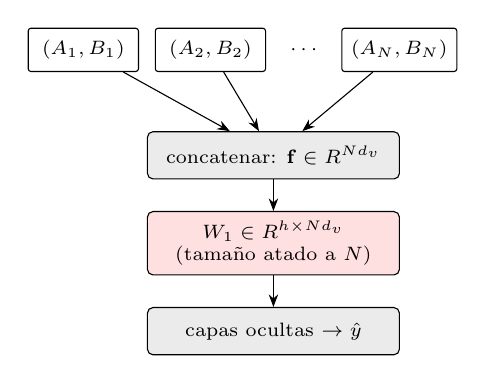
\begin{tikzpicture}[
    font=\scriptsize,
    box/.style={draw, rounded corners=1pt, minimum width=1.4cm, minimum height=0.55cm, align=center},
    op/.style={draw, fill=black!8, rounded corners=2pt, minimum width=3.2cm, minimum height=0.6cm, align=center},
    >={Stealth[length=1.6mm]}]
  \node[box] (v1) {$(A_1,B_1)$};
  \node[box, right=0.2cm of v1] (v2) {$(A_2,B_2)$};
  \node[right=0.18cm of v2] (vd) {$\cdots$};
  \node[box, right=0.18cm of vd] (vN) {$(A_N,B_N)$};
  \node[op, below=0.75cm of v2, xshift=0.8cm] (cat) {concatenar: $\mathbf{f}\in\mathbb{R}^{N d_v}$};
  \node[op, below=0.4cm of cat, fill=red!12] (w1) {$W_1\in\mathbb{R}^{h\times N d_v}$\\ (tama\~no atado a $N$)};
  \node[op, below=0.4cm of w1] (mlp) {capas ocultas $\to \hat y$};
  \draw[->] (v1) -- (cat); \draw[->] (v2) -- (cat);
  \draw[->] (vN) -- (cat);
  \draw[->] (cat) -- (w1); \draw[->] (w1) -- (mlp);
\end{tikzpicture}
\caption{Backbone MLP: una red por cada $N$.}
\label{fig:mlp}
\end{subfigure}
\hfill
\begin{subfigure}[b]{0.5\textwidth}
\centering
\begin{tikzpicture}[
    font=\scriptsize,
    box/.style={draw, rounded corners=1pt, minimum width=1.0cm, minimum height=0.55cm, align=center},
    phi/.style={draw, fill=blue!10, rounded corners=2pt, minimum width=1.0cm, minimum height=0.55cm, align=center},
    op/.style={draw, fill=black!8, rounded corners=2pt, minimum width=3.6cm, minimum height=0.6cm, align=center},
    >={Stealth[length=1.6mm]}]
  \node[box] (v1) {$x_1$};
  \node[box, right=0.45cm of v1] (v2) {$x_2$};
  \node[right=0.3cm of v2] (vd) {$\cdots$};
  \node[box, right=0.3cm of vd] (vN) {$x_N$};
  \node[phi, below=0.55cm of v1] (p1) {$\phi$};
  \node[phi, below=0.55cm of v2] (p2) {$\phi$};
  \node[phi, below=0.55cm of vN] (pN) {$\phi$};
  \node[op, below=0.7cm of p2, xshift=0.7cm, fill=green!12] (pool)
        {pooling (media): $z=\tfrac1N\sum_i \phi(x_i)$};
  \node[op, below=0.4cm of pool] (rho) {$\rho \to \hat y$};
  \draw[->] (v1) -- (p1); \draw[->] (v2) -- (p2); \draw[->] (vN) -- (pN);
  \draw[->] (p1) -- (pool); \draw[->] (p2) -- (pool); \draw[->] (pN) -- (pool);
  \draw[->] (pool) -- (rho);
  \node[draw, dashed, fit=(p1)(pN), inner sep=3pt,
        label={[font=\tiny]below:pesos compartidos}] {};
\end{tikzpicture}
\caption{Encoder Deep Sets: una red para todo $N$.}
\label{fig:deepsets}
\end{subfigure}
\caption{Comparación de los flujos de información. En la MLP (a), el número de vértices $N$
determina el tamaño de la primera capa $W_1$. En Deep Sets (b), la misma red $\phi$ se aplica
a cada vértice (pesos compartidos) y el \textit{pooling} colapsa el conjunto en un vector de
tamaño fijo; $N$ solo aparece en una operación sin parámetros.}
\label{fig:mlp_vs_deepsets}
\end{figure}

La Tabla~\ref{tab:transformaciones} detalla las transformaciones con sus dimensiones, para un
lote (\textit{batch}) de $B$ sistemas.

\begin{table}[ht]
\centering
\caption{Transformaciones del encoder Deep Sets (lote de $B$ sistemas).}
\label{tab:transformaciones}
\begin{tabular}{clc}
\toprule
Paso & Operación & Forma del tensor \\
\midrule
Entrada & $A_{\text{poly}},\,B_{\text{poly}}$ & $(B,N,n_x,n_x),\ (B,N,n_x,n_u)$ \\
1 & aplanar y concatenar por vértice & $(B,N,d_v)$ \\
2 & $\phi$ por vértice (pesos compartidos) & $(B,N,d)$ \\
3 & \textsc{pooling} (media sobre vértices) & $(B,d)$ \\
4 & $\rho$ & $(B,\dim y)$ \\
5 & desempaquetar a $(Q,Y)$ y proyectar (DR) & $(B,n_x,n_x),\ (B,n_u,n_x)$ \\
\bottomrule
\end{tabular}
\end{table}

El mecanismo preciso del paso~2 es el \textbf{peso compartido}: al aplicar una capa lineal
$\phi:\mathbb{R}^{d_v}\!\to\!\mathbb{R}^{d}$ a un tensor de forma $(B,N,d_v)$, la operación
actúa solo sobre la última dimensión y reutiliza la misma matriz de pesos para los $N$
vértices, de forma análoga a cómo una convolución comparte su núcleo a lo largo de las
posiciones de una imagen.

\subsection{Por qué una sola arquitectura sirve para todo $N$}
\label{subsec:porque_un_N}

Tres propiedades, visibles en~\eqref{eq:deepsets} y en la Figura~\ref{fig:mlp_vs_deepsets},
explican la invarianza a la cardinalidad:
\begin{enumerate}
    \item \textbf{$\phi$ opera por vértice.} Su matriz de pesos es
    $\mathbb{R}^{d\times d_v}$: su tamaño depende de la dimensión de \emph{un} vértice
    ($d_v$), nunca de $N$.
    \item \textbf{Pesos compartidos entre vértices.} Existe una única $\phi$ aplicada a todos,
    lo que elimina toda dependencia del orden y del número de vértices.
    \item \textbf{El \textsc{pooling} no tiene parámetros.} El promedio colapsa el conjunto de
    tamaño variable en un vector fijo de dimensión $d$; $N$ aparece únicamente en esa suma,
    así que jamás afecta el tamaño de ninguna capa entrenable.
\end{enumerate}
En consecuencia, el grafo de pesos completo ($\phi$, $\rho$ y la cabeza de salida) tiene
dimensiones fijas, y la misma red admite $N = 2,3,4,5,\dots$ sin modificación alguna.

\subsection{Invarianza a la permutación}
\label{subsec:invarianza}

El paso $\phi$ es \emph{equivariante} a permutación: reordenar los vértices reordena
idénticamente los embeddings $\phi(x_i)$. El \textsc{pooling} es una operación \emph{simétrica}
y convierte esa equivarianza en \textbf{invarianza}: el vector agregado $z$ es el mismo
independientemente del orden, y por ende $\hat y$ también. Se verificó numéricamente que
permutar los vértices altera la salida en $\sim 10^{-16}$ (el épsilon de máquina, esto es,
cero). Esta invarianza es el sesgo inductivo \emph{correcto}, pues coincide con la simetría
del conjunto factible de la LMI; la MLP, en cambio, debe aprenderla aproximadamente a partir
de los datos y no la garantiza.

\subsection{Elección de la agregación}
\label{subsec:pooling}

Las tres agregaciones simétricas usuales producen invarianza, pero difieren en escala. La
suma $\sum_i \phi(x_i)$ crece en magnitud con $N$, lo que dificulta el entrenamiento conjunto
con distintos $N$; el máximo (elemento a elemento) captura el vértice más extremo en cada
característica; y la \textbf{media} $\frac1N\sum_i \phi(x_i)$ normaliza por $N$, manteniendo la
escala del embedding constante a través de cardinalidades. Por esta razón se adopta el promedio
como operación de \textsc{pooling}.

\subsection{Garantía teórica y costo en parámetros}
\label{subsec:teoria_params}

La forma~\eqref{eq:deepsets} no es heurística: el teorema de Deep
Sets~\cite{zaheer2017deep} garantiza que es un \emph{aproximador universal} de la clase de
funciones invariantes a permutación, exactamente la clase a la que pertenece el mapa buscado.
La misma receta sustenta arquitecturas afines como PointNet~\cite{qi2017pointnet}, que emplea
agregación por máximo. Finalmente, la Tabla~\ref{tab:params} contrasta el costo: el MLP
necesita una primera capa cuyo tamaño crece con $N$ (y, por ende, un modelo por cada $N$),
mientras que Deep Sets emplea una primera capa de tamaño fijo y un único modelo para toda la
familia.

\begin{table}[ht]
\centering
\caption{Costo en parámetros de la primera capa ($n_x=3$, $n_u=1$, $h=128$).}
\label{tab:params}
\begin{tabular}{lccc}
\toprule
Arquitectura & Primera capa & ¿Depende de $N$? & N.º de modelos para $N\in\{2,3,4,5\}$ \\
\midrule
MLP        & $\mathrm{Linear}(N d_v \to h)$ & Sí ($3200$ si $N{=}2$; $7808$ si $N{=}5$) & 4 \\
Deep Sets  & $\mathrm{Linear}(d_v \to h)=1664$ & No & 1 \\
\bottomrule
\end{tabular}
\end{table}

En síntesis, reemplazar el backbone MLP por un encoder Deep Sets elimina la dependencia del
número de vértices interviniendo \emph{únicamente} en la etapa de codificación: la salida
\eqref{eq:dim_y} y la capa de proyección de Douglas--Rachford ya eran independientes de $N$,
por lo que se preserva intacto todo el aparato de factibilidad por construcción de LMI-Net.

%
%  Requiere las librerías TikZ de abajo. Si compilas con \include de este
%  archivo, las \usetikzlibrary funcionan aquí; idealmente muévelas al
%  preámbulo de MuñozPedro_MT.tex junto a \usepackage{tikz}.
% =====================================================================
\usetikzlibrary{positioning,arrows.meta,fit,backgrounds,calc}

\section{Encoder invariante al número de vértices: de la MLP a Deep Sets}
\label{sec:deepsets}

La arquitectura LMI-Net descrita en la Sección~\ref{sec:arquitectura_lminet} fija el número
de vértices del polítopo en $N=2$. Esta sección aborda la limitación estructural que impide
generalizar a un $N$ arbitrario y propone como solución un \textit{encoder} de conjunto
invariante a permutación y a cardinalidad, basado en la arquitectura \textit{Deep
Sets}~\cite{zaheer2017deep}.

\subsection{La entrada es un conjunto, no un vector}
\label{subsec:entrada_conjunto}

Un sistema politópico queda descrito por el \textbf{conjunto} de sus $N$ vértices
$\{(A_i, B_i)\}_{i=1}^{N}$, con $A_i \in \mathbb{R}^{n_x \times n_x}$ y
$B_i \in \mathbb{R}^{n_x \times n_u}$. Cada vértice aporta, por tanto,
\begin{equation}
    d_v \;=\; n_x^2 + n_x\,n_u
\end{equation}
escalares; para la topología de estudio ($n_x=3$, $n_u=1$) esto es $d_v = 9 + 3 = 12$.

Resulta esencial notar una \textbf{asimetría estructural} entre la entrada y la salida del
mapa que la red debe aprender. La salida es el certificado $(Q, Y)$ codificado en el vector
$y$, cuya dimensión
\begin{equation}
    \dim y \;=\; \tfrac{n_x(n_x+1)}{2} + n_u\,n_x
    \label{eq:dim_y}
\end{equation}
\textbf{no depende de $N$} (vale $6+3=9$ para todo $N$), porque se busca \emph{una sola}
función de Lyapunov común $V(x)=x^\top Q^{-1} x$ y \emph{una sola} ganancia $K = Y Q^{-1}$
válidas simultáneamente para todos los vértices (estabilizabilidad cuadrática). Además, el
conjunto factible de la LMI es idéntico ante cualquier reordenamiento de los vértices: la
entrada es un \emph{conjunto}, no una secuencia. El mapa a aprender es entonces
\begin{equation}
    \{(A_i,B_i)\}_{i=1}^{N} \;\longmapsto\; (Q, Y),
\end{equation}
es decir, \emph{un conjunto de tamaño variable hacia un vector de tamaño fijo, invariante a
permutación}.

\subsection{El cuello de botella del backbone MLP}
\label{subsec:cuello_mlp}

El backbone original construye un único vector aplanando y concatenando todos los vértices,
\begin{equation}
    \mathbf{f} \;=\; \big[\,\mathrm{vec}(A_1),\,\mathrm{vec}(B_1),\,\dots,\,
    \mathrm{vec}(A_N),\,\mathrm{vec}(B_N)\,\big] \in \mathbb{R}^{N d_v},
    \label{eq:features_mlp}
\end{equation}
y lo procesa con una red densa cuya primera capa es una matriz
$W_1 \in \mathbb{R}^{h \times N d_v}$ (con $h$ el ancho oculto). Esta construcción acarrea
dos problemas insalvables para un $N$ variable:

\begin{enumerate}
    \item \textbf{Dependencia dimensional.} El tamaño de $W_1$ está atado a $N$: una red
    entrenada con $N=2$ posee $W_1 \in \mathbb{R}^{h\times 24}$ y no puede siquiera recibir
    la entrada de un sistema con $N=3$ ($\mathbb{R}^{h\times 36}$). En consecuencia, se
    requiere \emph{una arquitectura distinta por cada valor de $N$}.
    \item \textbf{Dependencia del orden.} La concatenación~\eqref{eq:features_mlp} asigna una
    columna de pesos distinta a cada posición; la red aprende parámetros específicos para
    ``la entrada $(1,1)$ de $A$ del vértice $1$'', otros para el vértice $2$, etc. Pero los
    vértices forman un conjunto, de modo que la red malgasta capacidad intentando aprender
    una invarianza a permutación que no se le garantiza.
\end{enumerate}

El relleno con ceros (\textit{zero-padding}) hasta un $N_{\max}$ fijo no resuelve nada: no
restaura la invarianza a permutación, inyecta vértices espurios $A=0,\,B=0$ que la red
interpreta como restricciones reales, y sigue sin poder extrapolar a $N > N_{\max}$.

\subsection{El encoder Deep Sets}
\label{subsec:deepsets}

La idea central de Deep Sets es cambiar la unidad de procesamiento: en vez de operar sobre el
conjunto aplanado, se aplica una misma función a \emph{cada vértice por separado} y se agregan
los resultados con una operación simétrica. El teorema de representación
de~\cite{zaheer2017deep} establece que toda función continua invariante a permutación admite
la forma
\begin{equation}
    f\big(\{x_1,\dots,x_N\}\big) \;=\; \rho\!\left( \frac{1}{N}\sum_{i=1}^{N} \phi(x_i) \right),
    \label{eq:deepsets}
\end{equation}
donde $\phi$ y $\rho$ son perceptrones multicapa. Concretamente, para cada vértice se forma
$x_i = [\mathrm{vec}(A_i),\,\mathrm{vec}(B_i)] \in \mathbb{R}^{d_v}$; una MLP compartida
$\phi:\mathbb{R}^{d_v}\!\to\!\mathbb{R}^{d}$ lo lleva a un embedding; estos se agregan por
promedio en $z\in\mathbb{R}^{d}$; y una MLP $\rho:\mathbb{R}^{d}\!\to\!\mathbb{R}^{\dim y}$
produce la propuesta $\hat y$ que alimenta la capa de proyección de Douglas--Rachford, la cual
se conserva \emph{sin modificación}. La Figura~\ref{fig:mlp_vs_deepsets} contrasta ambos
flujos.

\begin{figure}[ht]
\centering
\begin{subfigure}[b]{0.46\textwidth}
\centering
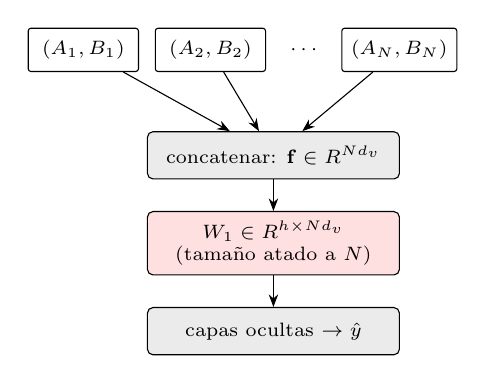
\begin{tikzpicture}[
    font=\scriptsize,
    box/.style={draw, rounded corners=1pt, minimum width=1.4cm, minimum height=0.55cm, align=center},
    op/.style={draw, fill=black!8, rounded corners=2pt, minimum width=3.2cm, minimum height=0.6cm, align=center},
    >={Stealth[length=1.6mm]}]
  \node[box] (v1) {$(A_1,B_1)$};
  \node[box, right=0.2cm of v1] (v2) {$(A_2,B_2)$};
  \node[right=0.18cm of v2] (vd) {$\cdots$};
  \node[box, right=0.18cm of vd] (vN) {$(A_N,B_N)$};
  \node[op, below=0.75cm of v2, xshift=0.8cm] (cat) {concatenar: $\mathbf{f}\in\mathbb{R}^{N d_v}$};
  \node[op, below=0.4cm of cat, fill=red!12] (w1) {$W_1\in\mathbb{R}^{h\times N d_v}$\\ (tama\~no atado a $N$)};
  \node[op, below=0.4cm of w1] (mlp) {capas ocultas $\to \hat y$};
  \draw[->] (v1) -- (cat); \draw[->] (v2) -- (cat);
  \draw[->] (vN) -- (cat);
  \draw[->] (cat) -- (w1); \draw[->] (w1) -- (mlp);
\end{tikzpicture}
\caption{Backbone MLP: una red por cada $N$.}
\label{fig:mlp}
\end{subfigure}
\hfill
\begin{subfigure}[b]{0.5\textwidth}
\centering
\begin{tikzpicture}[
    font=\scriptsize,
    box/.style={draw, rounded corners=1pt, minimum width=1.0cm, minimum height=0.55cm, align=center},
    phi/.style={draw, fill=blue!10, rounded corners=2pt, minimum width=1.0cm, minimum height=0.55cm, align=center},
    op/.style={draw, fill=black!8, rounded corners=2pt, minimum width=3.6cm, minimum height=0.6cm, align=center},
    >={Stealth[length=1.6mm]}]
  \node[box] (v1) {$x_1$};
  \node[box, right=0.45cm of v1] (v2) {$x_2$};
  \node[right=0.3cm of v2] (vd) {$\cdots$};
  \node[box, right=0.3cm of vd] (vN) {$x_N$};
  \node[phi, below=0.55cm of v1] (p1) {$\phi$};
  \node[phi, below=0.55cm of v2] (p2) {$\phi$};
  \node[phi, below=0.55cm of vN] (pN) {$\phi$};
  \node[op, below=0.7cm of p2, xshift=0.7cm, fill=green!12] (pool)
        {pooling (media): $z=\tfrac1N\sum_i \phi(x_i)$};
  \node[op, below=0.4cm of pool] (rho) {$\rho \to \hat y$};
  \draw[->] (v1) -- (p1); \draw[->] (v2) -- (p2); \draw[->] (vN) -- (pN);
  \draw[->] (p1) -- (pool); \draw[->] (p2) -- (pool); \draw[->] (pN) -- (pool);
  \draw[->] (pool) -- (rho);
  \node[draw, dashed, fit=(p1)(pN), inner sep=3pt,
        label={[font=\tiny]below:pesos compartidos}] {};
\end{tikzpicture}
\caption{Encoder Deep Sets: una red para todo $N$.}
\label{fig:deepsets}
\end{subfigure}
\caption{Comparación de los flujos de información. En la MLP (a), el número de vértices $N$
determina el tamaño de la primera capa $W_1$. En Deep Sets (b), la misma red $\phi$ se aplica
a cada vértice (pesos compartidos) y el \textit{pooling} colapsa el conjunto en un vector de
tamaño fijo; $N$ solo aparece en una operación sin parámetros.}
\label{fig:mlp_vs_deepsets}
\end{figure}

La Tabla~\ref{tab:transformaciones} detalla las transformaciones con sus dimensiones, para un
lote (\textit{batch}) de $B$ sistemas.

\begin{table}[ht]
\centering
\caption{Transformaciones del encoder Deep Sets (lote de $B$ sistemas).}
\label{tab:transformaciones}
\begin{tabular}{clc}
\toprule
Paso & Operación & Forma del tensor \\
\midrule
Entrada & $A_{\text{poly}},\,B_{\text{poly}}$ & $(B,N,n_x,n_x),\ (B,N,n_x,n_u)$ \\
1 & aplanar y concatenar por vértice & $(B,N,d_v)$ \\
2 & $\phi$ por vértice (pesos compartidos) & $(B,N,d)$ \\
3 & \textsc{pooling} (media sobre vértices) & $(B,d)$ \\
4 & $\rho$ & $(B,\dim y)$ \\
5 & desempaquetar a $(Q,Y)$ y proyectar (DR) & $(B,n_x,n_x),\ (B,n_u,n_x)$ \\
\bottomrule
\end{tabular}
\end{table}

El mecanismo preciso del paso~2 es el \textbf{peso compartido}: al aplicar una capa lineal
$\phi:\mathbb{R}^{d_v}\!\to\!\mathbb{R}^{d}$ a un tensor de forma $(B,N,d_v)$, la operación
actúa solo sobre la última dimensión y reutiliza la misma matriz de pesos para los $N$
vértices, de forma análoga a cómo una convolución comparte su núcleo a lo largo de las
posiciones de una imagen.

\subsection{Por qué una sola arquitectura sirve para todo $N$}
\label{subsec:porque_un_N}

Tres propiedades, visibles en~\eqref{eq:deepsets} y en la Figura~\ref{fig:mlp_vs_deepsets},
explican la invarianza a la cardinalidad:
\begin{enumerate}
    \item \textbf{$\phi$ opera por vértice.} Su matriz de pesos es
    $\mathbb{R}^{d\times d_v}$: su tamaño depende de la dimensión de \emph{un} vértice
    ($d_v$), nunca de $N$.
    \item \textbf{Pesos compartidos entre vértices.} Existe una única $\phi$ aplicada a todos,
    lo que elimina toda dependencia del orden y del número de vértices.
    \item \textbf{El \textsc{pooling} no tiene parámetros.} El promedio colapsa el conjunto de
    tamaño variable en un vector fijo de dimensión $d$; $N$ aparece únicamente en esa suma,
    así que jamás afecta el tamaño de ninguna capa entrenable.
\end{enumerate}
En consecuencia, el grafo de pesos completo ($\phi$, $\rho$ y la cabeza de salida) tiene
dimensiones fijas, y la misma red admite $N = 2,3,4,5,\dots$ sin modificación alguna.

\subsection{Invarianza a la permutación}
\label{subsec:invarianza}

El paso $\phi$ es \emph{equivariante} a permutación: reordenar los vértices reordena
idénticamente los embeddings $\phi(x_i)$. El \textsc{pooling} es una operación \emph{simétrica}
y convierte esa equivarianza en \textbf{invarianza}: el vector agregado $z$ es el mismo
independientemente del orden, y por ende $\hat y$ también. Se verificó numéricamente que
permutar los vértices altera la salida en $\sim 10^{-16}$ (el épsilon de máquina, esto es,
cero). Esta invarianza es el sesgo inductivo \emph{correcto}, pues coincide con la simetría
del conjunto factible de la LMI; la MLP, en cambio, debe aprenderla aproximadamente a partir
de los datos y no la garantiza.

\subsection{Elección de la agregación}
\label{subsec:pooling}

Las tres agregaciones simétricas usuales producen invarianza, pero difieren en escala. La
suma $\sum_i \phi(x_i)$ crece en magnitud con $N$, lo que dificulta el entrenamiento conjunto
con distintos $N$; el máximo (elemento a elemento) captura el vértice más extremo en cada
característica; y la \textbf{media} $\frac1N\sum_i \phi(x_i)$ normaliza por $N$, manteniendo la
escala del embedding constante a través de cardinalidades. Por esta razón se adopta el promedio
como operación de \textsc{pooling}.

\subsection{Garantía teórica y costo en parámetros}
\label{subsec:teoria_params}

La forma~\eqref{eq:deepsets} no es heurística: el teorema de Deep
Sets~\cite{zaheer2017deep} garantiza que es un \emph{aproximador universal} de la clase de
funciones invariantes a permutación, exactamente la clase a la que pertenece el mapa buscado.
La misma receta sustenta arquitecturas afines como PointNet~\cite{qi2017pointnet}, que emplea
agregación por máximo. Finalmente, la Tabla~\ref{tab:params} contrasta el costo: el MLP
necesita una primera capa cuyo tamaño crece con $N$ (y, por ende, un modelo por cada $N$),
mientras que Deep Sets emplea una primera capa de tamaño fijo y un único modelo para toda la
familia.

\begin{table}[ht]
\centering
\caption{Costo en parámetros de la primera capa ($n_x=3$, $n_u=1$, $h=128$).}
\label{tab:params}
\begin{tabular}{lccc}
\toprule
Arquitectura & Primera capa & ¿Depende de $N$? & N.º de modelos para $N\in\{2,3,4,5\}$ \\
\midrule
MLP        & $\mathrm{Linear}(N d_v \to h)$ & Sí ($3200$ si $N{=}2$; $7808$ si $N{=}5$) & 4 \\
Deep Sets  & $\mathrm{Linear}(d_v \to h)=1664$ & No & 1 \\
\bottomrule
\end{tabular}
\end{table}

En síntesis, reemplazar el backbone MLP por un encoder Deep Sets elimina la dependencia del
número de vértices interviniendo \emph{únicamente} en la etapa de codificación: la salida
\eqref{eq:dim_y} y la capa de proyección de Douglas--Rachford ya eran independientes de $N$,
por lo que se preserva intacto todo el aparato de factibilidad por construcción de LMI-Net.

%
%  Requiere las librerías TikZ de abajo. Si compilas con \include de este
%  archivo, las \usetikzlibrary funcionan aquí; idealmente muévelas al
%  preámbulo de MuñozPedro_MT.tex junto a \usepackage{tikz}.
% =====================================================================
\usetikzlibrary{positioning,arrows.meta,fit,backgrounds,calc}

\section{Encoder invariante al número de vértices: de la MLP a Deep Sets}
\label{sec:deepsets}

La arquitectura LMI-Net descrita en la Sección~\ref{sec:arquitectura_lminet} fija el número
de vértices del polítopo en $N=2$. Esta sección aborda la limitación estructural que impide
generalizar a un $N$ arbitrario y propone como solución un \textit{encoder} de conjunto
invariante a permutación y a cardinalidad, basado en la arquitectura \textit{Deep
Sets}~\cite{zaheer2017deep}.

\subsection{La entrada es un conjunto, no un vector}
\label{subsec:entrada_conjunto}

Un sistema politópico queda descrito por el \textbf{conjunto} de sus $N$ vértices
$\{(A_i, B_i)\}_{i=1}^{N}$, con $A_i \in \mathbb{R}^{n_x \times n_x}$ y
$B_i \in \mathbb{R}^{n_x \times n_u}$. Cada vértice aporta, por tanto,
\begin{equation}
    d_v \;=\; n_x^2 + n_x\,n_u
\end{equation}
escalares; para la topología de estudio ($n_x=3$, $n_u=1$) esto es $d_v = 9 + 3 = 12$.

Resulta esencial notar una \textbf{asimetría estructural} entre la entrada y la salida del
mapa que la red debe aprender. La salida es el certificado $(Q, Y)$ codificado en el vector
$y$, cuya dimensión
\begin{equation}
    \dim y \;=\; \tfrac{n_x(n_x+1)}{2} + n_u\,n_x
    \label{eq:dim_y}
\end{equation}
\textbf{no depende de $N$} (vale $6+3=9$ para todo $N$), porque se busca \emph{una sola}
función de Lyapunov común $V(x)=x^\top Q^{-1} x$ y \emph{una sola} ganancia $K = Y Q^{-1}$
válidas simultáneamente para todos los vértices (estabilizabilidad cuadrática). Además, el
conjunto factible de la LMI es idéntico ante cualquier reordenamiento de los vértices: la
entrada es un \emph{conjunto}, no una secuencia. El mapa a aprender es entonces
\begin{equation}
    \{(A_i,B_i)\}_{i=1}^{N} \;\longmapsto\; (Q, Y),
\end{equation}
es decir, \emph{un conjunto de tamaño variable hacia un vector de tamaño fijo, invariante a
permutación}.

\subsection{El cuello de botella del backbone MLP}
\label{subsec:cuello_mlp}

El backbone original construye un único vector aplanando y concatenando todos los vértices,
\begin{equation}
    \mathbf{f} \;=\; \big[\,\mathrm{vec}(A_1),\,\mathrm{vec}(B_1),\,\dots,\,
    \mathrm{vec}(A_N),\,\mathrm{vec}(B_N)\,\big] \in \mathbb{R}^{N d_v},
    \label{eq:features_mlp}
\end{equation}
y lo procesa con una red densa cuya primera capa es una matriz
$W_1 \in \mathbb{R}^{h \times N d_v}$ (con $h$ el ancho oculto). Esta construcción acarrea
dos problemas insalvables para un $N$ variable:

\begin{enumerate}
    \item \textbf{Dependencia dimensional.} El tamaño de $W_1$ está atado a $N$: una red
    entrenada con $N=2$ posee $W_1 \in \mathbb{R}^{h\times 24}$ y no puede siquiera recibir
    la entrada de un sistema con $N=3$ ($\mathbb{R}^{h\times 36}$). En consecuencia, se
    requiere \emph{una arquitectura distinta por cada valor de $N$}.
    \item \textbf{Dependencia del orden.} La concatenación~\eqref{eq:features_mlp} asigna una
    columna de pesos distinta a cada posición; la red aprende parámetros específicos para
    ``la entrada $(1,1)$ de $A$ del vértice $1$'', otros para el vértice $2$, etc. Pero los
    vértices forman un conjunto, de modo que la red malgasta capacidad intentando aprender
    una invarianza a permutación que no se le garantiza.
\end{enumerate}

El relleno con ceros (\textit{zero-padding}) hasta un $N_{\max}$ fijo no resuelve nada: no
restaura la invarianza a permutación, inyecta vértices espurios $A=0,\,B=0$ que la red
interpreta como restricciones reales, y sigue sin poder extrapolar a $N > N_{\max}$.

\subsection{El encoder Deep Sets}
\label{subsec:deepsets}

La idea central de Deep Sets es cambiar la unidad de procesamiento: en vez de operar sobre el
conjunto aplanado, se aplica una misma función a \emph{cada vértice por separado} y se agregan
los resultados con una operación simétrica. El teorema de representación
de~\cite{zaheer2017deep} establece que toda función continua invariante a permutación admite
la forma
\begin{equation}
    f\big(\{x_1,\dots,x_N\}\big) \;=\; \rho\!\left( \frac{1}{N}\sum_{i=1}^{N} \phi(x_i) \right),
    \label{eq:deepsets}
\end{equation}
donde $\phi$ y $\rho$ son perceptrones multicapa. Concretamente, para cada vértice se forma
$x_i = [\mathrm{vec}(A_i),\,\mathrm{vec}(B_i)] \in \mathbb{R}^{d_v}$; una MLP compartida
$\phi:\mathbb{R}^{d_v}\!\to\!\mathbb{R}^{d}$ lo lleva a un embedding; estos se agregan por
promedio en $z\in\mathbb{R}^{d}$; y una MLP $\rho:\mathbb{R}^{d}\!\to\!\mathbb{R}^{\dim y}$
produce la propuesta $\hat y$ que alimenta la capa de proyección de Douglas--Rachford, la cual
se conserva \emph{sin modificación}. La Figura~\ref{fig:mlp_vs_deepsets} contrasta ambos
flujos.

\begin{figure}[ht]
\centering
\begin{subfigure}[b]{0.46\textwidth}
\centering
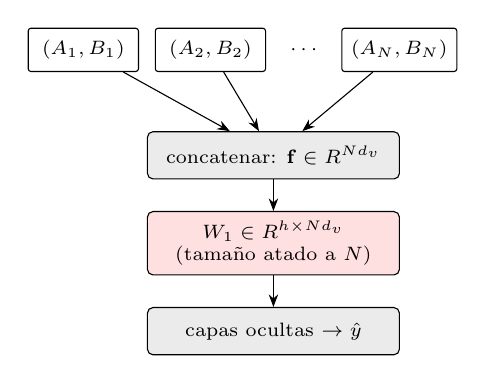
\begin{tikzpicture}[
    font=\scriptsize,
    box/.style={draw, rounded corners=1pt, minimum width=1.4cm, minimum height=0.55cm, align=center},
    op/.style={draw, fill=black!8, rounded corners=2pt, minimum width=3.2cm, minimum height=0.6cm, align=center},
    >={Stealth[length=1.6mm]}]
  \node[box] (v1) {$(A_1,B_1)$};
  \node[box, right=0.2cm of v1] (v2) {$(A_2,B_2)$};
  \node[right=0.18cm of v2] (vd) {$\cdots$};
  \node[box, right=0.18cm of vd] (vN) {$(A_N,B_N)$};
  \node[op, below=0.75cm of v2, xshift=0.8cm] (cat) {concatenar: $\mathbf{f}\in\mathbb{R}^{N d_v}$};
  \node[op, below=0.4cm of cat, fill=red!12] (w1) {$W_1\in\mathbb{R}^{h\times N d_v}$\\ (tama\~no atado a $N$)};
  \node[op, below=0.4cm of w1] (mlp) {capas ocultas $\to \hat y$};
  \draw[->] (v1) -- (cat); \draw[->] (v2) -- (cat);
  \draw[->] (vN) -- (cat);
  \draw[->] (cat) -- (w1); \draw[->] (w1) -- (mlp);
\end{tikzpicture}
\caption{Backbone MLP: una red por cada $N$.}
\label{fig:mlp}
\end{subfigure}
\hfill
\begin{subfigure}[b]{0.5\textwidth}
\centering
\begin{tikzpicture}[
    font=\scriptsize,
    box/.style={draw, rounded corners=1pt, minimum width=1.0cm, minimum height=0.55cm, align=center},
    phi/.style={draw, fill=blue!10, rounded corners=2pt, minimum width=1.0cm, minimum height=0.55cm, align=center},
    op/.style={draw, fill=black!8, rounded corners=2pt, minimum width=3.6cm, minimum height=0.6cm, align=center},
    >={Stealth[length=1.6mm]}]
  \node[box] (v1) {$x_1$};
  \node[box, right=0.45cm of v1] (v2) {$x_2$};
  \node[right=0.3cm of v2] (vd) {$\cdots$};
  \node[box, right=0.3cm of vd] (vN) {$x_N$};
  \node[phi, below=0.55cm of v1] (p1) {$\phi$};
  \node[phi, below=0.55cm of v2] (p2) {$\phi$};
  \node[phi, below=0.55cm of vN] (pN) {$\phi$};
  \node[op, below=0.7cm of p2, xshift=0.7cm, fill=green!12] (pool)
        {pooling (media): $z=\tfrac1N\sum_i \phi(x_i)$};
  \node[op, below=0.4cm of pool] (rho) {$\rho \to \hat y$};
  \draw[->] (v1) -- (p1); \draw[->] (v2) -- (p2); \draw[->] (vN) -- (pN);
  \draw[->] (p1) -- (pool); \draw[->] (p2) -- (pool); \draw[->] (pN) -- (pool);
  \draw[->] (pool) -- (rho);
  \node[draw, dashed, fit=(p1)(pN), inner sep=3pt,
        label={[font=\tiny]below:pesos compartidos}] {};
\end{tikzpicture}
\caption{Encoder Deep Sets: una red para todo $N$.}
\label{fig:deepsets}
\end{subfigure}
\caption{Comparación de los flujos de información. En la MLP (a), el número de vértices $N$
determina el tamaño de la primera capa $W_1$. En Deep Sets (b), la misma red $\phi$ se aplica
a cada vértice (pesos compartidos) y el \textit{pooling} colapsa el conjunto en un vector de
tamaño fijo; $N$ solo aparece en una operación sin parámetros.}
\label{fig:mlp_vs_deepsets}
\end{figure}

La Tabla~\ref{tab:transformaciones} detalla las transformaciones con sus dimensiones, para un
lote (\textit{batch}) de $B$ sistemas.

\begin{table}[ht]
\centering
\caption{Transformaciones del encoder Deep Sets (lote de $B$ sistemas).}
\label{tab:transformaciones}
\begin{tabular}{clc}
\toprule
Paso & Operación & Forma del tensor \\
\midrule
Entrada & $A_{\text{poly}},\,B_{\text{poly}}$ & $(B,N,n_x,n_x),\ (B,N,n_x,n_u)$ \\
1 & aplanar y concatenar por vértice & $(B,N,d_v)$ \\
2 & $\phi$ por vértice (pesos compartidos) & $(B,N,d)$ \\
3 & \textsc{pooling} (media sobre vértices) & $(B,d)$ \\
4 & $\rho$ & $(B,\dim y)$ \\
5 & desempaquetar a $(Q,Y)$ y proyectar (DR) & $(B,n_x,n_x),\ (B,n_u,n_x)$ \\
\bottomrule
\end{tabular}
\end{table}

El mecanismo preciso del paso~2 es el \textbf{peso compartido}: al aplicar una capa lineal
$\phi:\mathbb{R}^{d_v}\!\to\!\mathbb{R}^{d}$ a un tensor de forma $(B,N,d_v)$, la operación
actúa solo sobre la última dimensión y reutiliza la misma matriz de pesos para los $N$
vértices, de forma análoga a cómo una convolución comparte su núcleo a lo largo de las
posiciones de una imagen.

\subsection{Por qué una sola arquitectura sirve para todo $N$}
\label{subsec:porque_un_N}

Tres propiedades, visibles en~\eqref{eq:deepsets} y en la Figura~\ref{fig:mlp_vs_deepsets},
explican la invarianza a la cardinalidad:
\begin{enumerate}
    \item \textbf{$\phi$ opera por vértice.} Su matriz de pesos es
    $\mathbb{R}^{d\times d_v}$: su tamaño depende de la dimensión de \emph{un} vértice
    ($d_v$), nunca de $N$.
    \item \textbf{Pesos compartidos entre vértices.} Existe una única $\phi$ aplicada a todos,
    lo que elimina toda dependencia del orden y del número de vértices.
    \item \textbf{El \textsc{pooling} no tiene parámetros.} El promedio colapsa el conjunto de
    tamaño variable en un vector fijo de dimensión $d$; $N$ aparece únicamente en esa suma,
    así que jamás afecta el tamaño de ninguna capa entrenable.
\end{enumerate}
En consecuencia, el grafo de pesos completo ($\phi$, $\rho$ y la cabeza de salida) tiene
dimensiones fijas, y la misma red admite $N = 2,3,4,5,\dots$ sin modificación alguna.

\subsection{Invarianza a la permutación}
\label{subsec:invarianza}

El paso $\phi$ es \emph{equivariante} a permutación: reordenar los vértices reordena
idénticamente los embeddings $\phi(x_i)$. El \textsc{pooling} es una operación \emph{simétrica}
y convierte esa equivarianza en \textbf{invarianza}: el vector agregado $z$ es el mismo
independientemente del orden, y por ende $\hat y$ también. Se verificó numéricamente que
permutar los vértices altera la salida en $\sim 10^{-16}$ (el épsilon de máquina, esto es,
cero). Esta invarianza es el sesgo inductivo \emph{correcto}, pues coincide con la simetría
del conjunto factible de la LMI; la MLP, en cambio, debe aprenderla aproximadamente a partir
de los datos y no la garantiza.

\subsection{Elección de la agregación}
\label{subsec:pooling}

Las tres agregaciones simétricas usuales producen invarianza, pero difieren en escala. La
suma $\sum_i \phi(x_i)$ crece en magnitud con $N$, lo que dificulta el entrenamiento conjunto
con distintos $N$; el máximo (elemento a elemento) captura el vértice más extremo en cada
característica; y la \textbf{media} $\frac1N\sum_i \phi(x_i)$ normaliza por $N$, manteniendo la
escala del embedding constante a través de cardinalidades. Por esta razón se adopta el promedio
como operación de \textsc{pooling}.

\subsection{Garantía teórica y costo en parámetros}
\label{subsec:teoria_params}

La forma~\eqref{eq:deepsets} no es heurística: el teorema de Deep
Sets~\cite{zaheer2017deep} garantiza que es un \emph{aproximador universal} de la clase de
funciones invariantes a permutación, exactamente la clase a la que pertenece el mapa buscado.
La misma receta sustenta arquitecturas afines como PointNet~\cite{qi2017pointnet}, que emplea
agregación por máximo. Finalmente, la Tabla~\ref{tab:params} contrasta el costo: el MLP
necesita una primera capa cuyo tamaño crece con $N$ (y, por ende, un modelo por cada $N$),
mientras que Deep Sets emplea una primera capa de tamaño fijo y un único modelo para toda la
familia.

\begin{table}[ht]
\centering
\caption{Costo en parámetros de la primera capa ($n_x=3$, $n_u=1$, $h=128$).}
\label{tab:params}
\begin{tabular}{lccc}
\toprule
Arquitectura & Primera capa & ¿Depende de $N$? & N.º de modelos para $N\in\{2,3,4,5\}$ \\
\midrule
MLP        & $\mathrm{Linear}(N d_v \to h)$ & Sí ($3200$ si $N{=}2$; $7808$ si $N{=}5$) & 4 \\
Deep Sets  & $\mathrm{Linear}(d_v \to h)=1664$ & No & 1 \\
\bottomrule
\end{tabular}
\end{table}

En síntesis, reemplazar el backbone MLP por un encoder Deep Sets elimina la dependencia del
número de vértices interviniendo \emph{únicamente} en la etapa de codificación: la salida
\eqref{eq:dim_y} y la capa de proyección de Douglas--Rachford ya eran independientes de $N$,
por lo que se preserva intacto todo el aparato de factibilidad por construcción de LMI-Net.
